%!TEX root = ../thesis.tex

\chapter{闪电氮氧化物产率的估算} \label{chapter:PE}

\section{清洁地区(北极)}

\subsection{闪电的分布}
\subsection{反演闪电氮氧化物的步骤}
\subsection{闪电氮氧化物的聚类}
\subsection{闪电氮氧化物浓度与其他氮氧化物源的对比}
\subsection{闪电氮氧化物的寿命及产率}
\subsection{不确定性分析}


\section{污染地区(中国及美国大陆)}

\subsection{模式设置}

使用的WRF-Chem版本为3.5.1,水平网格大小为12 km $\times$ 12 km (图 ??(a)),垂直层数为29层,时间步长为72 s。
气象条件的初始场和边界场为时间分辨率3小时的北美区域再分析(NARR)数据集,每3小时应用一次边界条件和四维数据分析(FDDA)逼近,
其中温度、水汽和水平风以0.0003 s$^{-1}$ 的系数逼近\citep{Laughner.2017}。
微物理过程采用Lin方案\citep{Lin.1983},积云参数化为Grell 3D方案\citep{Grell.1993a,Grell.2002a},长波辐射采用RRTM方案\citep{Iacono.2008},短波辐射采用Goddard方案,陆面过程使用Noah陆面模式\citep{Koren.1999},边界层采用YSU方案\citep{Hong.2006}。
闪电参数化采用基于对流参数化的中性浮力水平\citep{Pickering.1992},云闪与地闪的比例基于\citet{Boccippio.2001}.

采用臭氧和相关化学示踪剂模型第4版(MOZART-4;\citet{Emmons.2010})的输出场作为化学的初始场和边界场。
人为排放由2011年美国国家排放清单(NEI)驱动,并根据环境保护署年度总排放量,按模拟的年份进行调整\citep{EPA.2015}。
生物排放使用MEGAN源,化学机制是区域大气化学机制第2版(RACM2;\citet{Goliff.2013}),并由\citet{Browne.2014}和\citet{Schwantes.2015}进行了更新。
此外,LNO$_x$参数化采用每次闪电产生200 mol NO,调整因子为1,以下简称“1$\times$200 mol NO per flash”)。
基于\citet{Ott.2010}的双峰型闪电NO(LNO)廓线\citep{Laughner.2017}被用作 WRF-Chem中LNO的垂直分布,而LNO和LNO$_2$廓线是指有和没有闪电的模拟之间垂直廓线的差异。


\subsection{反演闪电氮氧化物的步骤}

首先我们使用恒定值网格化法,将公式(\ref{eq:AMF_LNO2})所得的LNO$_x$垂直柱密度(V$_{\textrm{NO$_x$}}$)分配至0.05$^{\circ}$ $\times$ 0.05$^{\circ}$网格\citep{Kuhlmann.2014}。
接着在 1$^{\circ}$ $\times$ 1$^{\circ}$的网格中进行分析,要求每个网格至少有50个有效的0.05$^{\circ}$ $\times$ 0.05$^{\circ}$网格数据,从而最小化噪点数据。
具体LNO$_x$的主要计算步骤如下。

云辐射分数(CRF,CRF $\geq$ 70\%,CRF $\geq$ 90\%,CRF = 100\%)和 云压(CP,CP $\leq$ 650 hPa)是OMI像素是否包含深对流云的判断标准\citep{Ziemke.2009,Choi.2014,Pickering.2016}。
不同CRF对LNO$_x$产品的影响将在\ref{subsec:criteria}节探讨。
此外,我们将另一个云分数 (CF) 标准应用于 WRF-Chem 的模拟结果,以确保对流被成功模拟。
具体而言,CF是由 Xu-Randall 方法计算的 350--400 hPa 之间的最大云分数\citep{Xu.1996,Strode.2017}。
选择350--400 hPa的大气层,可避免模拟高云中的偏差。
我们选择\citet{Strode.2017}建议的 CF $\geq$ 40\%来判断模拟所处的网格是多云或晴空。

除了云特性之外,OMI能探测到新生LNO$_x$的另一条件为一段时间内有足够的闪电或闪击。
其中,时间窗口 (t$_{window}$) 是 OMI 过境之前的时间段。
\citet{Lapierre.2020}利用1$^{\circ}$ $\times$ 1$^{\circ}$网格的对角线长度和OMI过境时美国大陆上空500--100 hPa的平均风速计算得到t$_{window}$为2.4 h。
同时,\citet{Lapierre.2020}定义在t$_{window}$时间段内,至少发生2400次闪电或8160次闪击的网格才能提供足够的LNO$_x$给OMI探测。
\citet{Bucsela.2019}的研究表明,低频率的闪电具有更高的LNO$_x$产率(PE),而该段数据在\citet{Lapierre.2020}研究中被剔除。
通过比较使用每个网格至少2400次闪电和至少1次闪电的标准所得结果,我们也得到相同的结论(图\ref{fig:flash_threshold})。
由于我们的研究重点是开发一种新的空气质量转换因子(AMF),并将计算结果与使用类似闪电阈值的其他产品进行比较\citep{Pickering.2016,Lapierre.2020},
因此我们接下来使用相同的至少2400次闪电标准来进行结果分析。


\begin{figure}[h]
    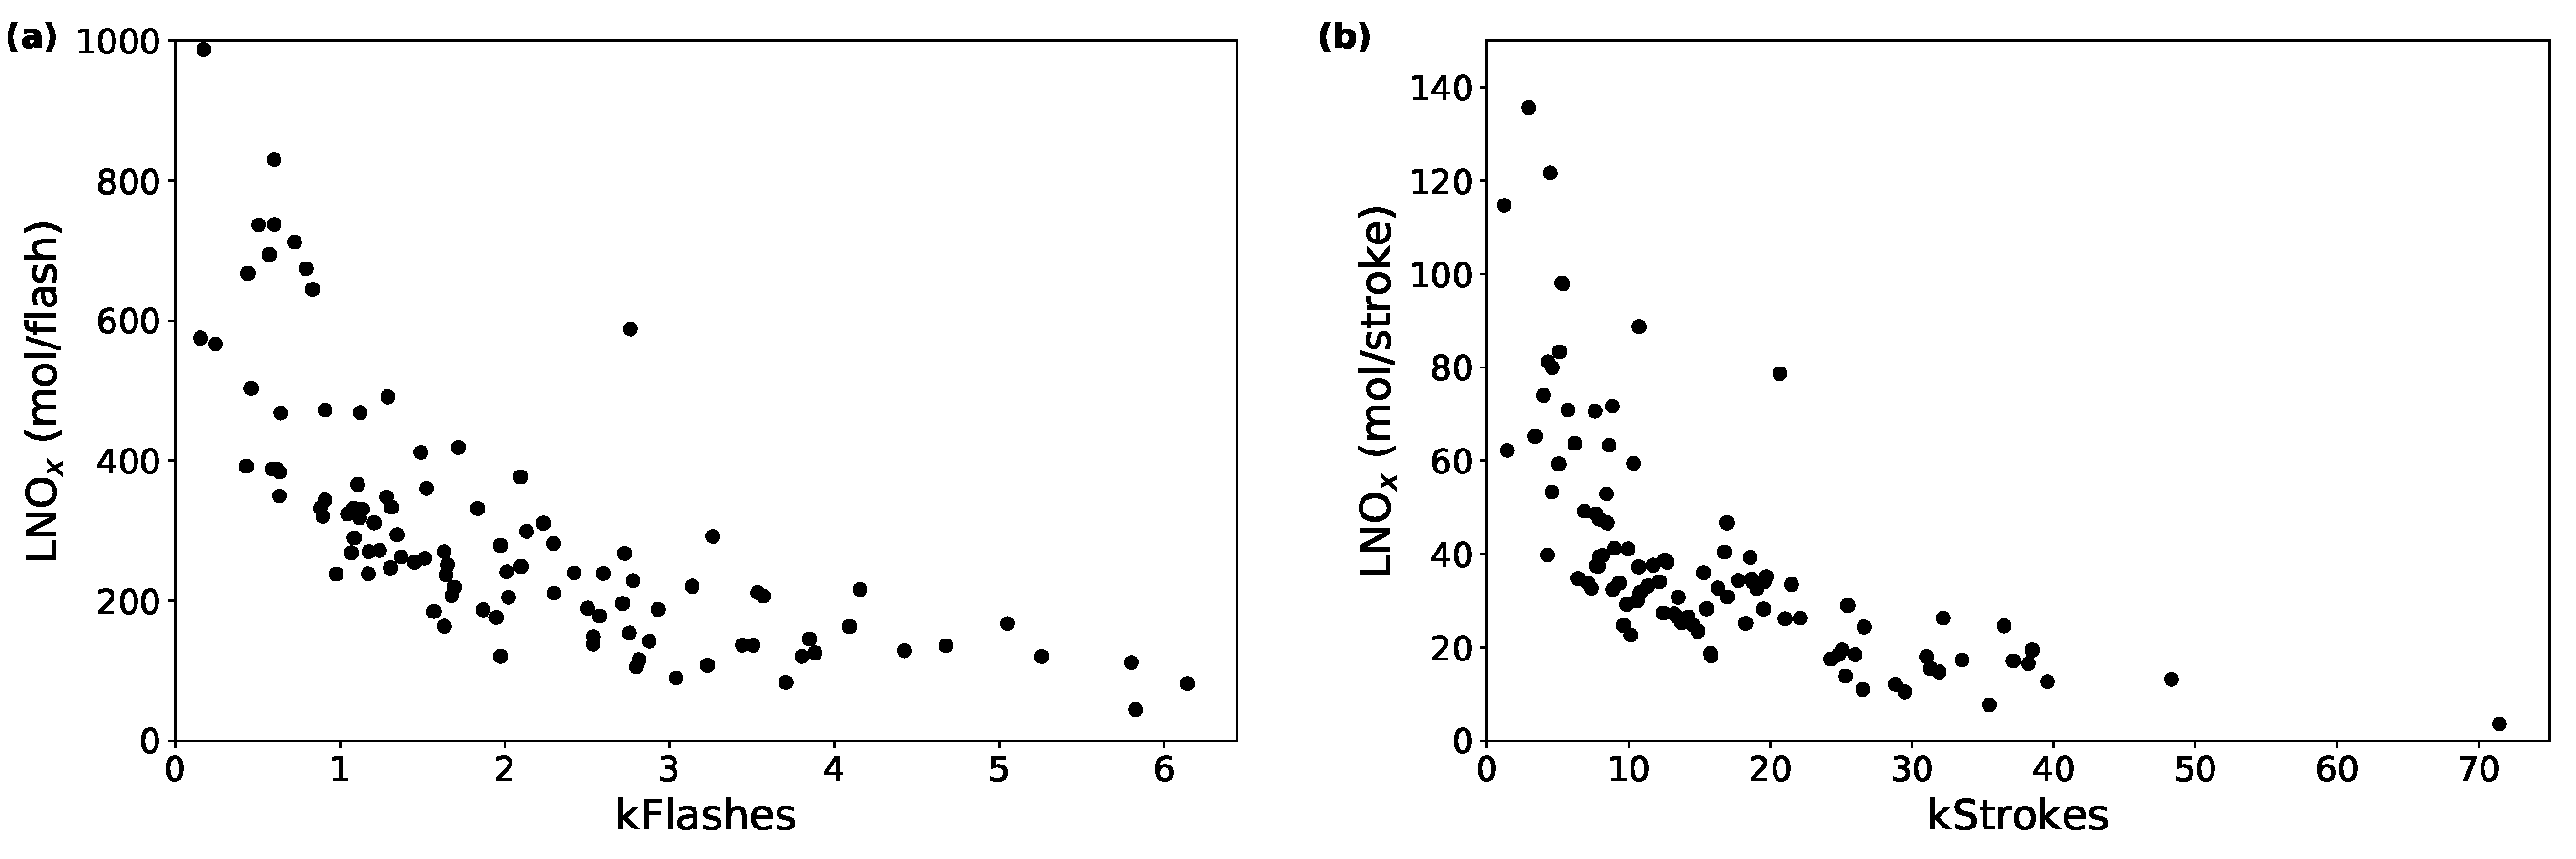
\includegraphics[width=15cm]{./figures/flash_threshold.pdf}
    \caption{
    (a) 每日 LNO$_x$ 产率与 ENTLN 总闪的关系,筛选条件为CRF $\geq$ 90\% 且1$^{\circ}$ $\times$ 1$^{\circ}$网格中至少有1次闪电。
     (b) 与 (a) 相同,但针对闪击。\\
    (a) Daily LNO$_\textrm{x}$ production efficiencies versus ENTLN total flashes data, with CRF $\geq$ 90\% and a flash threshold of 1 flash box$^{-1}$.
    (b) Same as (a) but for strokes.}
    \label{fig:flash_threshold}
\end{figure}


为确保WRF-Chem成功模拟闪电并考虑到闪电参数化的不确定性,我们将每个1$^{\circ}$ $\times$ 1$^{\circ}$网格模拟的总闪电(TL)阈值设置为1000,该阈值低于ENTLN闪电观测使用的阈值。
针对除LNO$_2$之外的其他NO$_2$源,我们定义了模拟的云上闪电NO$_2$柱密度(LNO$_2$Vis)与云上NO$_2$柱密度(NO$_2$Vis)之比,来判断OMI是否可以检测到足够的LNO$_2$。
该比率$\geq$50\%表明云层上方超过一半的NO$_x$具有LNO$_x$源。
此外,还需考虑氧化有关的NO$_2$寿命。
\citet{Nault.2017}的研究表明NO$_2$在对流附近的寿命($\tau$)为$\approx$3 h,故NO$_2$的初始值可由方程式(\ref{eq:inition})求解。

\begin{equation} \label{eq:inition}
NO_2(0) = NO_2(OMI) \times e^{0.5t/\tau}
\end{equation}

其中$NO_2(0)$是在时间 t=0 排放的NO$_2$摩尔数,$NO_2(OMI)$是在 OMI 过境时间测得的NO$_2$摩尔数,
0.5t是穿过网格的时间,即1.2 h,(假设闪电出现在每个1$^{\circ}$ $\times$ 1$^{\circ}$网格的中心)。
每个网格的V$_\textrm{LNO$_x$}$为网格中所有0.05$^{\circ}$ $\times$ 0.05$^{\circ}$像素的V$_\textrm{LNO$_x$}$平均值,
然后乘以网格的面积得到LNO$_x$摩尔数。

最后,有两种方法可用于估算季节性平均LNO$_2$每闪电、LNO$_x$每闪电、LNO$_x$每闪击和 LNO$_x$每闪击:

(1)求和法,将LNO$_x$的总和除以5--8月中每个1$^{\circ}$ $\times$ 1$^{\circ}$网格里发生的闪电或闪击总数;

(2)线性回归方法,将线性回归应用于LNO$_x$和每日闪电或闪击的平均值。

\subsection{适合反演闪电氮氧化物的条件} \label{subsec:criteria}

根据上节定义的条件,我们定义了六种不同的筛选条件组合(表),并使用线性回归方法(表)应用于原始数据。

\begin{table*}[h]
\scriptsize
\caption{本研究中使用的标准的缩写定义\\Table \ref{table:Abbreviations}Definitions of the abbreviations for the criteria used in this study.}
\begin{tabular}{ll}
\hline
\textbf{缩写} & \textbf{全称 [来源]} \\
\hline
CRF                             & Cloud radiance fraction [OMI] \\
CP                              & Cloud optical pressure [OMI] \\
CF                              & Cloud fraction [WRF-Chem] \\
TL                              & Total lightning flashes [WRF-Chem] \\
ratio                           & modeled LNO$_2$Vis / modeled NO$_2$Vis [WRF-Chem] \\
CRF$\alpha$\_ENTLN                    & CRF $\geq$ $\alpha$ + ENTLN flashes(strokes) $\geq$ 2400(8160) [ENTLN]\\
CRF$\alpha$\_CF40\_ENTLN              & CRF $\geq$ $\alpha$ + ENTLN flashes(strokes) $\geq$ 2400(8160) + CF $\geq$ 40\% \\
CRF$\alpha$\_ENTLN\_TL1000            & CRF $\geq$ $\alpha$ + ENTLN flashes(strokes) $\geq$ 2400(8160) + TL $\geq$ 1000 \\
CRF$\alpha$\_CF40\_ENTLN\_TL1000      & CRF $\geq$ $\alpha$ + ENTLN flashes(strokes) $\geq$ 2400(8160) + CF $\geq$ 40\% + TL $\geq$ 1000 \\
CRF$\alpha$\_ENTLN\_TL1000\_ratio50   & CRF $\geq$ $\alpha$ + ENTLN flashes(strokes) $\geq$ 2400(8160) + TL $\geq$ 1000 + ratio $\geq$ 50\% \\
CRF$\alpha$\_CF40\_ENTLN\_TL1000\_ratio50 & CRF $\geq$ $\alpha$ + ENTLN flashes(strokes) $\geq$ 2400(8160) + CF $\geq$ 40\% + TL $\geq$ 1000 + ratio $\geq$ 50\% \\
CRF$\alpha$\_ENTLN1(3.4)\_TL1\_ratio50    & CRF $\geq$ $\alpha$ + ENTLN flashes(strokes) $\geq$ 1(3.4) + TL $\geq$ 1 + ratio $\geq$ 50\% \\
\hline
\multicolumn{2}{l}{$^{*}$$\alpha$有三种选择:70\%、90\%以及100\%} \\
\multicolumn{2}{l}{$^{*}$$\alpha$ has three options: 70\%, 90\% and 100\%}
\end{tabular}
\label{table:Abbreviations}
\end{table*}


\begin{table*}[h]
\scriptsize
\caption{根据表\ref{table:Abbreviations}中的定义得到的LNO$_\textrm{x}$产率\\Table \ref{table:conditions} LNO$_\textrm{x}$ production efficiencies for different combinations of criteria defined in Table \ref{table:Abbreviations}.}
\begin{tabular}{lccccc}
\hline
\textbf{条件$^1$} & \textbf{ENTLN类型$^2$} & \textbf{LNO$_\textrm{x}$/flash or LNO$_\textrm{x}$/stroke} & \textbf{R值} & \textbf{截距 (10$^{6}$mol)} & \textbf{天数$^3$} \\
\hline
CRF90\_ENTLN                        & Flash  & 52.1 $\pm$ 51.1 & 0.20 & 0.21  & 99 \\
CRF90\_CF40\_ENTLN                  & Flash  & 84.2 $\pm$ 31.5 & 0.54 & -0.04 & 70 \\
CRF90\_ENTLN\_TL1000                & Flash  & 61.9 $\pm$ 49.1 & 0.27 & 0.33  & 83 \\
CRF90\_CF40\_ENTLN\_TL1000          & Flash  & 63.4 $\pm$ 52.9 & 0.38 & 0.26  & 38 \\
CRF90\_ENTLN\_TL1000\_ratio50       & Flash  & 54.5 $\pm$ 48.1 & 0.25 & 0.39  & 81 \\
CRF90\_CF40\_ENTLN\_TL1000\_ratio50 & Flash  & 90.0 $\pm$ 65.0 & 0.46 & 0.15  & 32 \\
CRF90\_ENTLN                        & Stroke & 6.7 $\pm$ 4.1 & 0.31 & 0.23  & 102 \\
CRF90\_CF40\_ENTLN                  & Stroke & 10.3 $\pm$ 3.6 & 0.55 & 0.08 & 79 \\
CRF90\_ENTLN\_TL1000                & Stroke & 7.5 $\pm$ 5.1 & 0.29 & 0.38  & 94 \\
CRF90\_CF40\_ENTLN\_TL1000          & Stroke & 8.6 $\pm$ 6.2 & 0.39 & 0.27  & 46 \\
CRF90\_ENTLN\_TL1000\_ratio50       & Stroke & 7.0 $\pm$ 4.8 & 0.29 & 0.42  & 93 \\
CRF90\_CF40\_ENTLN\_TL1000\_ratio50 & Stroke & 8.9 $\pm$ 7.0 & 0.39 & 0.31  & 40 \\
\hline
\multicolumn{6}{l}{$^1$定义见表\ref{table:Abbreviations}。}\\
\multicolumn{6}{l}{$^2$ENTLN阈值为OMI过境前2.4小时内,1$^{\circ}$ $\times$ 1$^{\circ}$网格中闪电至少2400次和闪击至少8160次。}\\
\multicolumn{6}{l}{$^3$2014年5--8月中有效的天数。} \\
\multicolumn{6}{l}{$^1$These conditions are defined in Table \ref{table:Abbreviations}.} \\
\multicolumn{6}{l}{$^2$The thresholds of ENTLN data are 2400 flashes box$^{-1}$ and 8160 strokes box$^{-1}$ during the period of 2.4 h before OMI overpass time.} \\
\multicolumn{6}{l}{$^3$The number of valid days with specific criteria in MJJA 2014.}
\label{table:conditions}
\end{tabular}
\end{table*}


在CRF90\_ENTLN条件下,有效闪电(闪击)数据对应共有99(102)天。
以闪电类ENTLN数据为例,在 CRF90\_ENTLN\_TL1000\_ratio50 条件下,有效天数从 99 减少至 81,而LNO$_x$产率从 52.1$\pm$51.1 mol每闪电增加到 54.5$\pm$48.1 mol每闪电。
该结果与 CRF90\_ENTLN\_TL1000 条件下所得的结果几乎相同。
尽管这表明TL筛选条件已足够严格,但最好包括云上LNO$_2$占比的筛选条件,以防不同的AMF方法中存在一些例外情况。
由于 CF $\geq$ 40\% 会导致有效数据和产率急剧下降,因此我们仅仅使用 CRF 对数据进行筛选。
最后,我们选择至少2400次闪电或至少8160次闪击,TL $\geq$ 1000 和云上LNO$_2$占比 $\geq$ 50\% 作为阈值,来探索三种不同 CRF 条件(CRF $\geq$ 70\%、CRF $\geq$ 90\% 和 CRF = 100\%)对 LNO$_x$ 估算产生的影响(表\ref{table:CRFs})。
当CRF 标准从 70\% 增加到 90\% 和 100\%时,针对闪电类型的LNO$_x$产率 从35.7$\pm$36.8 mol每闪电增加到 54.5$\pm$48.1 mol每闪电,然后再降低到20.8$\pm$37.4 mol每闪电,而针对闪击类型的LNO$_x$产率从4.1$\pm$3.9 mol每闪击提高到 7.0$\pm$4.8 mol每闪击,然后再次下降到2.6$\pm$4.0 mol每闪击(表\ref{table:CRFs})。
当 CRF 从 90\% 增加到 100\% 时LNO$_x$ PE 降低,这是因为闪电密度较高而 LNO$_x$ 较少。
CRF 从 70\% 增加到 90\% 引起的 LNO$_x$ PE 增加与\citet{Pickering.2016}的结果相反。
这是由于我们的方法中考虑了从边界层传输的 NO$_2$ 污染的影响。
虽然在 CRF > 70\% 的地区经常观察到 NO$_x$ 增强\citet{Pickering.2016},但考虑到中低浓度 NO$_2$ 的污染并与\citet{Pickering.2016}和\citet{Lapierre.2020}的结果进行比较,以下分析将基于 CRF $\geq$ 90\% 标准进行讨论分析。

\begin{table*}[h]
\scriptsize
\caption{在相同ENTLN阈值,TL $\geq$ 1000 和云上LNO$_2$占比 $\geq$ 50\%的条件下,不同云辐射分数阈值对应的LNO$_\textrm{x}$产率 \\ LNO$_\textrm{x}$ production efficiencies for different thresholds of CRF with coincident ENTLN data, TL $\geq$ 1000 and ratio $\geq$ 50\%.}
\begin{tabular}{cccccc}
\hline
\textbf{云辐射分数 (\%)} & \textbf{ENTLN类型$^1$} & \textbf{LNO$_\textrm{x}$每闪电 or LNO$_\textrm{x}$每闪击} & \textbf{R值} & \textbf{截距 (10$^{5}$mol)} & \textbf{天数$^2$} \\
\hline
70  & 闪电  & 35.7  $\pm$ 36.8 & 0.21 & 4.91 & 85 \\
90  & 闪电  & 54.5  $\pm$ 48.1 & 0.25 & 3.90 & 81 \\
100 & 闪电  & 20.8  $\pm$ 37.4 & 0.13 & 5.67 & 71 \\
70  & 闪击 & 4.1   $\pm$ 3.9  & 0.21 & 5.16 & 96 \\
90  & 闪击 & 7.0   $\pm$ 4.8  & 0.29 & 4.16 & 93 \\
100 & 闪击 & 2.6   $\pm$ 4.0  & 0.14 & 5.41 & 82 \\
\hline
\multicolumn{6}{l}{$^1$ENTLN阈值为 OMI f过境前 2.4 小时内每个网格闪电至少 2400 次 或 闪击至少8160 次。}\\
\multicolumn{6}{l}{$^2$2014年5--8月对应筛选条件下有效天数。} \\
\multicolumn{6}{l}{$^1$The thresholds of ENTLN data are 2400 flashes box$^{-1}$ and 8160 strokes box$^{-1}$ during the period of 2.4 h before OMI overpass time.}\\
\multicolumn{6}{l}{$^2$The number of valid days with specific criteria in MJJA 2014.}
\end{tabular}
\label{table:CRFs}
\end{table*}

\subsection{不同反演方法的对比}

\citet{Lapierre.2020}基于 BEHR NO$_2$ 产品得出 LNO$_2$ 产量,
为了使本研究的结果与\citet{Pickering.2016}和\citet{Lapierre.2020}的结果具有可比性,我们选择 NO$_2$  而不是 NO$_x$  来计算每次闪电的产量(产率,PE)。
在图\ref{fig:pe_timeseries}中,根据 CRF $\geq$ 90\% 和每 2.4 h 2400次闪电的阈值,绘制了2014年5--8月美国大陆每天 NO$_2$Vis、LNO$_2$Vis、LNO$_2$ 和 LNO$_2$Clean 产率的时间序列图。
其中,LNO$_2$ PE 大多在 20 至 80 mol每闪电的范围内,LNO$_2$Vis PE 小于 LNO$_2$ PE,因为后者在云层下含有 LNO$_2$。
\citet{Pickering.2016}的GMI模拟结果表明,25\%--30\%的LNO$_x$柱密度位于 云压(CP)以下,而我们的 WRF-Chem 模拟结果显示该比例为 56$\pm$20\%。
云属性对 LNO$_x$ PE 的影响将在第\ref{susbec:china_uncertainty}节中更详细地讨论。
总体而言,估算得到的每日PE顺序为LNO$_2$Clean > LNO$_2$ > NO$_2$Vis > LNO$_2$Vis。
通过NO$_2$Vis 和 LNO$_2$Vis 估算得到的PE之间的差异($\Delta$PE)表明有一定量的背景 NO$_2$ 存在于云层之上。
总体而言,该 $\Delta$PE 的趋势与 NO$_2$Vis 和 LNO$_2$Clean 之间的$\Delta$PE 一致。
当区域污染严重时(NO$_2$Vis 和 LNO$_2$Vis 之间的 $\Delta$PE > 200\%),基于 NO$_2$Vis 和 LNO$_2$Clean 的 PE 被显著高估。
换言之,NO$_2$Vis 和 LNO$_2$Clean 对背景 NO$_2$ 更为敏感。
且在高污染地区,NO$_2$Vis 的高估程度大于 LNO$_2$Clean,而在其他大多数地区通常相反。

\begin{figure}[h]
\centering
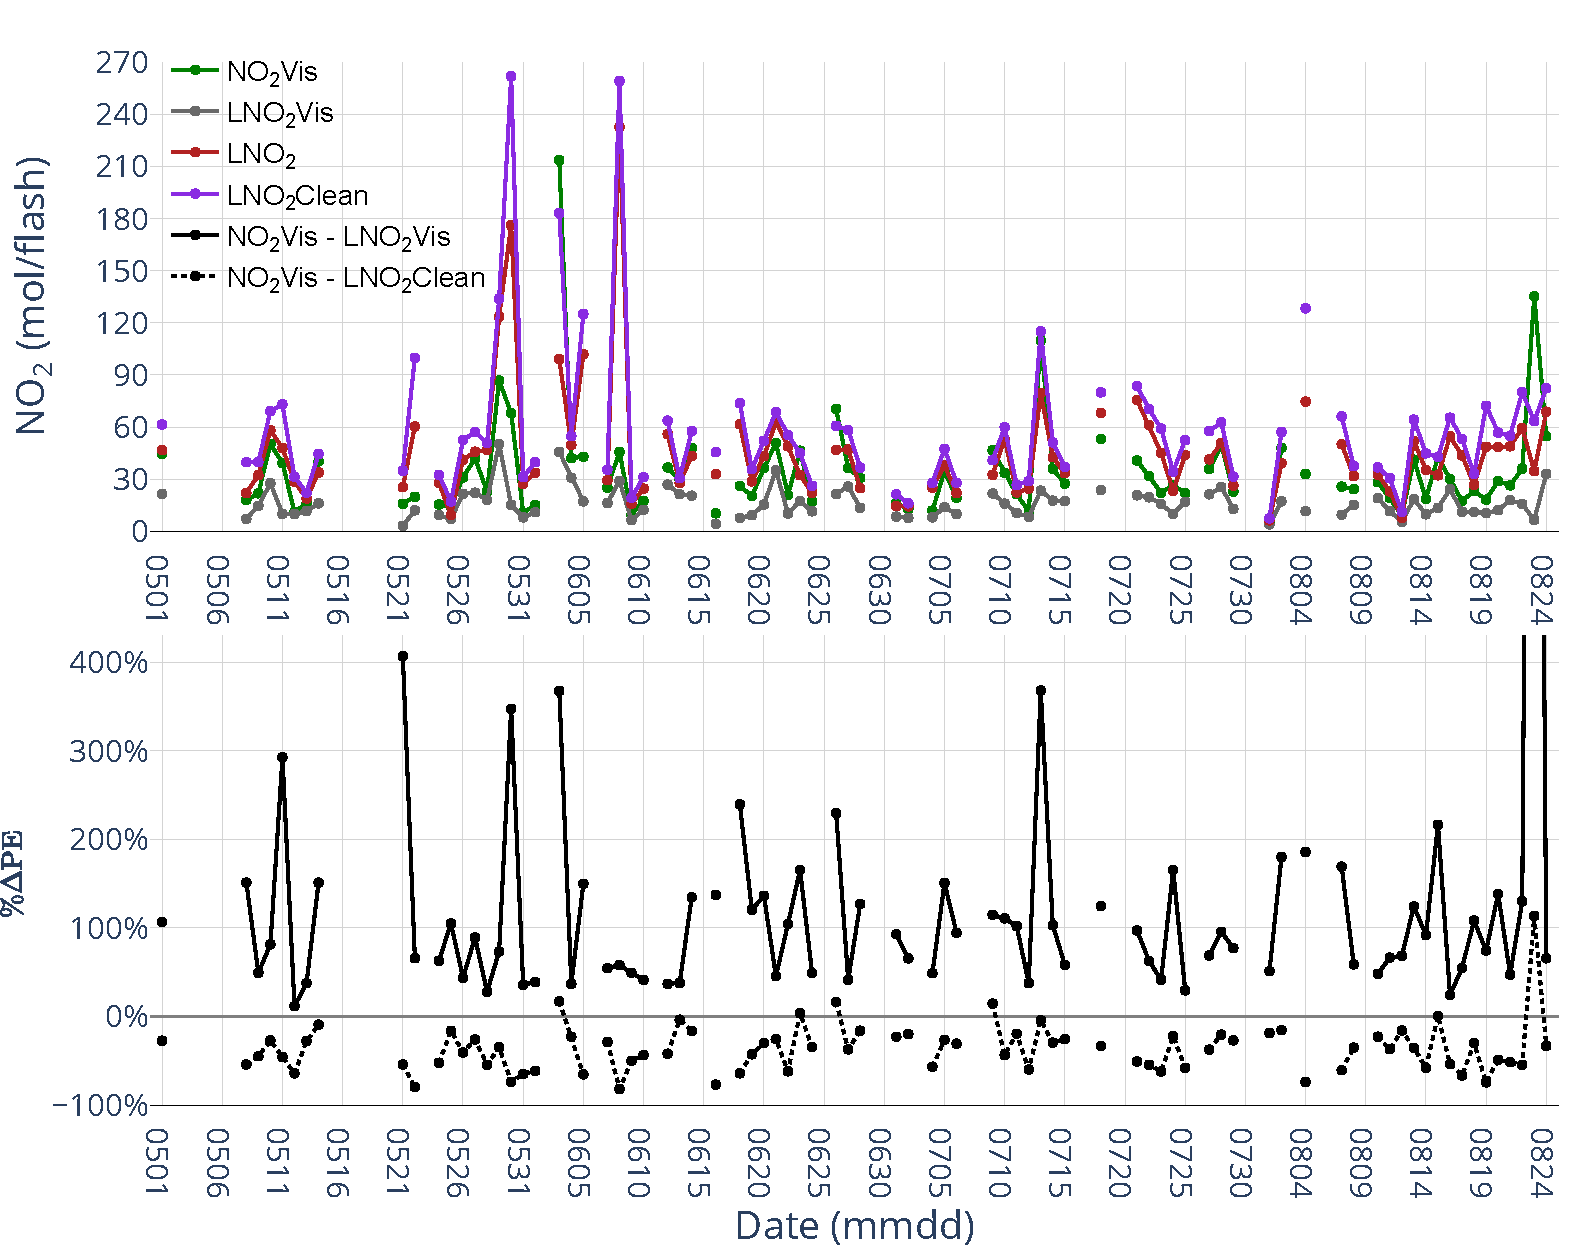
\includegraphics[width=12cm]{./figures/pe_timeseries.pdf}
\caption{(top) Time series of NO$_\textrm{2}$Vis, LNO$_\textrm{2}$Vis, LNO$_\textrm{2}$ and LNO$_\textrm{2}$Clean production per day over the CONUS for MJJA 2014 with CRF $\geq$ 90\% and a flash threshold of 2400 flashes per 2.4 h.
(bottom) Time series of the percent differences between NO$_\textrm{2}$Vis and LNO$_\textrm{2}$Vis and the percent differences between NO$_\textrm{2}$Vis and LNO$_\textrm{2}$Clean with CRF $\geq$ 90\%.
The value of black dot on August 23 (not shown) is 1958\%.}
\label{fig:pe_timeseries}
\end{figure}


\subsection{背景氮氧化物浓度对反演的影响}

\subsection{不确定性分析} \label{susbec:china_uncertainty}

\section{本章小结}
